%Professor, a seção de Sistemas de Controle ainda não finalizada e, portanto, seu conteúdo não é exibido aqui.
Um sistema de controle é, segundo \citeonline[p.~2]{Dorf2011}, uma interconexão de componentes formando uma configuração de sistema que vai fornecer uma resposta desejada. Todo sistema de controle tem, como objetivo, atuar sobre um determinado processo, o qual pode ser representado por um bloco que representa a relação entre entrada e saída do sistema, como mostrado na Figura \ref{fig:process}.

\begin{figure}[!htb]
    \centering
    \caption{Diagrama representando um processo}
    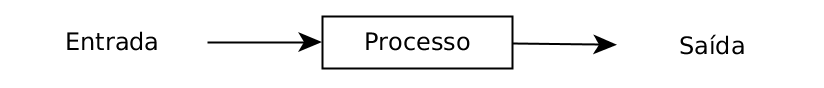
\includegraphics[width=0.7\textwidth]{./04-figuras/fund_teorica/process}
    \fonte{Adaptado de \citeonline[p.~2]{Dorf2011}}
    \label{fig:process}
\end{figure}

O controle sobre um processo pode assumir duas formas distintas: malha aberta ou malha fechada sendo que um sistema de controle em malha aberta é composto, além do processo, por um controlador e um atuador para se obter a resposta desejada sem o uso de realimentação \cite[p.~2]{Dorf2011}. Um exemplo de sistema deste tipo é mostrado na Figura \ref{fig:open_loop_control_system}.

\begin{figure}[!htb]
    \centering
    \caption{Diagrama representando um sistema de controle em malha aberta}
    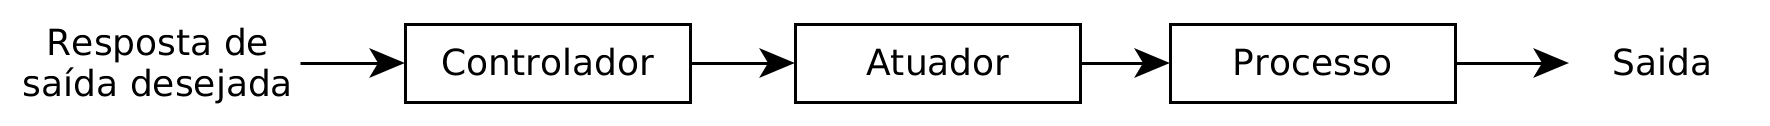
\includegraphics[width=0.95\textwidth]{./04-figuras/fund_teorica/open_loop_control_system}
    \fonte{Adaptado de \citeonline[p.~2]{Dorf2011}}
    \label{fig:open_loop_control_system}
\end{figure}

Em oposição a um sistema de controle em malha aberta, um em malha fechada encorpora, além dos componentes que aquele inclui, uma medição da saída atual para ser comparada com a saída desejada para o processo. Um exemplo de um sistema de controle em malha fechada simples é mostrado na Figura \ref{fig:closed_loop_control_system}. Os sistemas em malha fechada possuem várias vantagens sobre os em malha aberta como, por exemplo, a capacidade de rejeitar distúrbios externos e melhorar a atenuação de ruídos nas medições, componentes estes que são inevitáveis em aplicações no mundo real \cite[p.~3]{Dorf2011}.

\begin{figure}[!htb]
    \centering
    \caption{Diagrama representando um sistema de controle em malha fechada}
    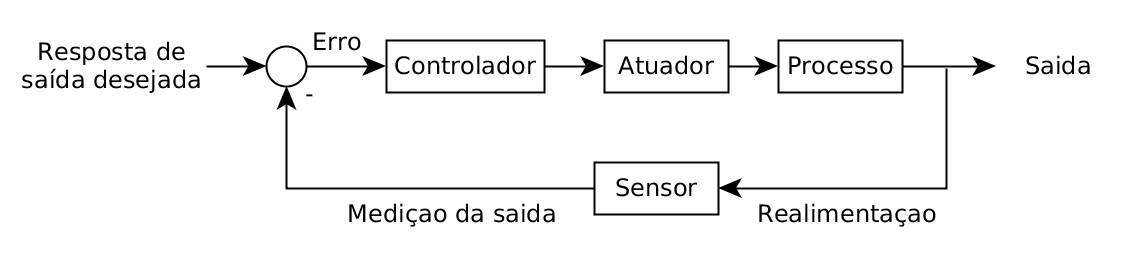
\includegraphics[width=0.95\textwidth]{./04-figuras/fund_teorica/closed_loop_control_system}
    \fonte{Adaptado de \citeonline[p.~3]{Dorf2011}}
    \label{fig:closed_loop_control_system}
\end{figure}

Como já foi visto, um processo representa a relação entre a entrada e a saída de um sistema sendo que há diferentes formas de fazê-lo. As próximas seções discutem as principais delas: as funções de transferência e a representação no espaço de estados.

\subsection{Funções de Transferência}
\label{subsec:fundamentacaoTeorica-tfs}

%Ogata 15 do pdf; Dorf 65 do pdf
A função de transferência de um sistema representa a relação que descreve as dinâmicas do sistema em questão e é definida pela razão entre as transformadas de Laplace das variáveis de saída e de entrada com todas as condições iniciadas definidas como zero \cite[p.~65]{Dorf2011}. A forma de uma função de transferência é dada a seguir:
\begin{center}
$G(s) = \frac{Y(s)}{X(s)}$
\end{center}
em que $G(s)$ é a função de transferência que descreve o sistema, $Y(s)$ é a transformada de Laplace da variável de saída do sistema e $X(s)$ é a transformada de Laplace da variável de entrada, ambas considerando as condições iniciais definidas como zero.

Apesar de ser amplamente utilizada, o uso de funções de transferência tem certas limitações. As transformadas de Laplace só podem ser utilizadas sobre sistemas descritos por equações e diferencias lineares e sem parâmetros variantes no tempo e, portanto, o uso das funções de transferência se restringem aos casos em que estas condições são satisfeitas.

Além da representação a partir de funções de transferência, uma forma alternativa de representar as dinâmicas do sistema é a representação no espaço de estados.



\subsection{Espaço de Estados}
\label{subsec:fundamentacaoTeorica-ss}

%Ogata 29 do pdf (digrma de blocos na pag 32); Dorf 165 do pdf
A representação de um sistema dinâmico no espaço de estados descreve um sistema a partir das seguintes equações :
\begin{center}\label{eq:k1}
%$\dot{x}(t)=A(t)x(t)+B(t)u(t)$ \\
%$y(t)=C(t)x(t)+D(t)u(t)$
$\dot{x}=Ax+Bu$ \\
$y=Cx+Du$
\end{center}
%em que $A(t)$ é a matriz de estados, $B(t)$ a matriz de entrada, $C(t)$ a matriz de saída, $D(t)$ a matriz de transmissão direta, $x$ é o vetor de variáveis de estado, $u$ o vetor de entradas e $y$ o vetor de saídas. A Figura \ref{fig:ss_diagram} exibe um diagrama de blocos para a representação em espaço de estados definida.
em que $A$ é a matriz de estados, $B$ a matriz de entrada, $C$ a matriz de saída, $D$ a matriz de transmissão direta, $x$ é o vetor de variáveis de estado, $u$ o vetor de entradas e $y$ o vetor de saídas. A Figura \ref{fig:ss_diagram} exibe um diagrama de blocos para a representação em espaço de estados definida.

\begin{figure}[!htb]
    \centering
    \caption{Diagrama de blocos de um sistema linear e contínuo tempo representado no espaço de estados}
    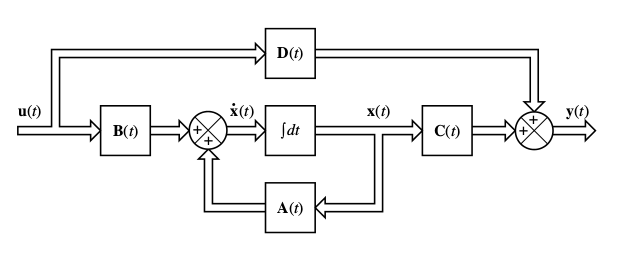
\includegraphics[width=0.9\textwidth]{./04-figuras/fund_teorica/ss_diagram}
    \fonte{\citeonline[p.~32]{Ogata2010}}
    \label{fig:ss_diagram}
\end{figure}

A representação no espaço de estados oferece uma ferramenta poderosa para a manipulação da representação do sistema, permitindo que as variáveis de estado sejam representadas de forma independente entre si a partir do processo de desacoplamento delas.

O processo de desacoplamento de variáveis de estado é baseado em ferramentas matemáticas aplicando manipulações sobre frações parciais. A partir deste processo, por exemplo, o sistema mostrado na Figura \ref{fig:ss_coupled}, que representa um sistema de controle de um motor CC com velocidade como saída e é representado pela função de transferência:
\begin{equation}
G(s)=\frac{30(s+1)}{(s+5)(s+2)(s+3)}
\end{equation}
pode ser representado por uma função de transferência do tipo:
\begin{equation}
G(s)=\frac{q(s)}{(s-s_1)(s-s_2)(s-s_3)}
\end{equation}
cuja resposta é ditada por $s_1$, $s_2$ e $s_3$. Utilizando a expansão de frações parciais, pode-se representar a mesma função de transferência por \cite[p.~183]{Dorf2011}:
\begin{equation}
T(s)=\frac{k_1}{s+5}+\frac{k_2}{s+2}+\frac{k_3}{s+3}
\end{equation}

\begin{figure}[!htb]
    \centering
    \caption{Diagrama de blocos representando o controle de um motor CC com velocidade como saída}
    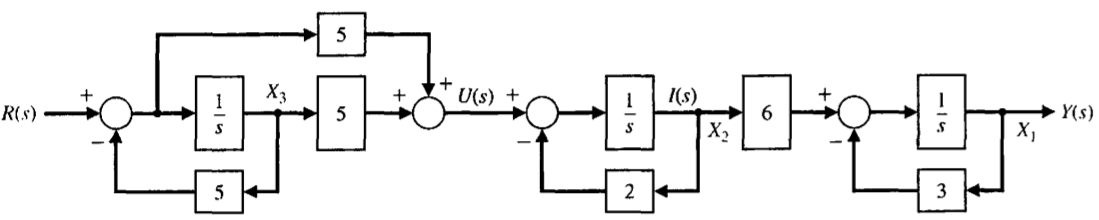
\includegraphics[width=1\textwidth]{./04-figuras/fund_teorica/ss_coupled_blocks}
    \fonte{\citeonline[p.~182]{Dorf2011}}
    \label{fig:ss_coupled}
\end{figure}

A partir de manipulações matemáticas relacionadas à expansão de frações parciais, constata-se que $k_1=-20$, $k_2=-10$ e $k_3=30$ \cite[p.~182]{Dorf2011}. Com isto, o sistema exibido na Figura \ref{fig:ss_coupled} pode ser representado como mostrado na Figura \ref{fig:ss_decoupled} que, como se pode ver, trata $X_1$, $X_2$ e $X_3$ de forma completamente independente e somando suas respectivas contribuições em $Y(s)$. Desta forma, pode-se ver claramente como cada variável de estado contribui para a saída ($Y(s)$) a partir de uma dada entrada ($X(s)$).

\begin{figure}[!htb]
    \centering
    \caption{Diagrama de blocos representando o controle de um motor CC com velocidade como saída e implementando desacoplamento das variáveis de estado}
    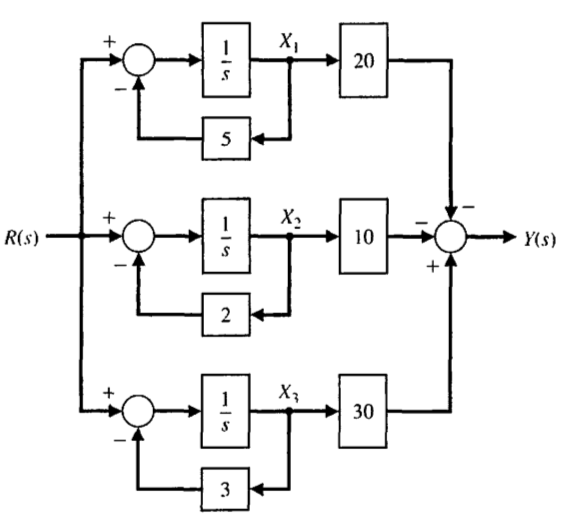
\includegraphics[width=0.6\textwidth]{./04-figuras/fund_teorica/ss_decoupled_blocks}
    \fonte{\citeonline[p.~182]{Dorf2011}}
    \label{fig:ss_decoupled}
\end{figure}










%No contexto deste trabalho, utilizou-se um sistema de controle em malha fechada no qual o processo a ser controlado diz respeito a um quadrotor. Além disto, os controladores utilizados foram de tipos bastante específicos: fuzzy e neuro-fuzzy, temas que são tratados nas próximas seções.

%Desacoplamento: Dorf pag 182 do pdf
